\documentclass[9pt,xcolor={table}]{beamer}
\setbeamertemplate{caption}[numbered]
\usetheme[white]{Illinois}
%\title[short title]{long title}
\title[HALEU Transitions]{Investigation of Impacts of Deploying 
Reactors Fueled by High Assay Low Enriched Uranium}
\subtitle{Preliminary Exam}
\author[Amanda M. Bachmann]{Amanda M. Bachmann\\ Advanced Reactors and Fuel Cycles Group}
%\author[Kathryn D. Huff]{Kathryn D. Huff\\Advanced Reactors and Fuel Cycles Group}
\date[09.08.2022]{September 8, 2022}
\institute[UIUC]{University of Illinois at Urbana-Champaign}


%\usepackage[table]{xcolor}
\usepackage{amsfonts}
\usepackage{amsmath}
\usepackage{xspace}
\usepackage{graphicx}
\usepackage{caption}
\usepackage{subcaption}
\usepackage{booktabs} % nice rules for tables
\usepackage{microtype} % if using PDF
\usepackage{bigints}

\graphicspath{{../images/}}

\newcommand{\units}[1] {\:\text{#1}}%
\newcommand{\SN}{S$_N$}%{S$_\text{N}$}%{$S_N$}%
\newcommand{\Cyclus}{\textsc{Cyclus}\xspace} %
\newcommand{\Cycamore}{\textsc{Cycamore}\xspace} %
\DeclareMathOperator{\erf}{erf}
%I need some complimentary error functions... 
\DeclareMathOperator{\erfc}{erfc}
%Those icons in the references are terrible looking
\setbeamertemplate{bibliography item}[text]

%%%% Acronym support

\usepackage[acronym,toc]{glossaries}
\input{../acros}

\usepackage{tikz}
\usetikzlibrary{shapes.geometric, arrows, backgrounds}
\usetikzlibrary{positioning, arrows, decorations, shapes, matrix, fit, tikzmark}

\tikzstyle{agent} = [rectangle, rounded corners, minimum width=0.1cm, minimum height=0.2cm,text centered, draw=black, fill=blue!30]
\tikzstyle{transition} = [rectangle, rounded corners, minimum width=0.1cm, minimum height=0.2cm,text centered, draw=black, fill=red!30]
\tikzstyle{arrow} = [thick,->,>=stealth]

\tikzstyle{region} = [rectangle, rounded corners, minimum width=0.1cm, minimum height=0.2cm,text centered, draw=black, fill=green!30]
\tikzstyle{institution} = [rectangle, rounded corners, minimum width=0.1cm, minimum height=0.2cm,text centered, draw=black, fill=red!30]
\tikzstyle{facility} = [rectangle, rounded corners, minimum width=0.1cm, minimum height=0.2cm,text centered, draw=black, fill=blue!30]
\tikzstyle{connect} = [thick,-]

\def\firstcircle{(0,0) circle (2cm)}
\def\secondcircle{(60:3cm) circle (2cm)}
\def\thirdcircle{(0:3cm) circle (2cm)}
\makeglossaries

%try to get rid of header on title page\dots
\makeatletter
    \newenvironment{withoutheadline}{
        \setbeamertemplate{headline}[default]
        \def\beamer@entrycode{\vspace*{-\headheight}}
    }{}
\makeatother

\makeatother
\setbeamertemplate{footline}
{
  \leavevmode%
  \hbox{%
    \rightline{\insertframenumber{} / \inserttotalframenumber\hspace*{1ex}}
  }%
  \vskip0pt%
}
\makeatletter
\begin{document}
%%%%%%%%%%%%%%%%%%%%%%%%%%%%%%%%%%%%%%%%%%%%%%%%%%%%%%%%%%%%%
%% From uw-beamer Here's a handy bit of code to place at 
%% the beginning of your presentation (after \begin{document}):
\newcommand*{\alphabet}{ABCDEFGHIJKLMNOPQRSTUVWXYZabcdefghijklmnopqrstuvwxyz}
\newlength{\highlightheight}
\newlength{\highlightdepth}
\newlength{\highlightmargin}
\setlength{\highlightmargin}{2pt}
\settoheight{\highlightheight}{\alphabet}
\settodepth{\highlightdepth}{\alphabet}
\addtolength{\highlightheight}{\highlightmargin}
\addtolength{\highlightdepth}{\highlightmargin}
\addtolength{\highlightheight}{\highlightdepth}
\newcommand*{\Highlight}{\rlap{\textcolor{HighlightBackground}{\rule[-\highlightdepth]{\linewidth}{\highlightheight}}}}
\colorlet{lightblue}{blue!40!}
\definecolor{lightorange}{HTML}{FAA21A}
\colorlet{lightpink}{red!20!}

\tikzset{   
        every picture/.style={remember picture,baseline},
        every node/.style={anchor=base,align=center,outer sep=1.5pt},
        every path/.style={thick},
        }

\newcommand\marktopleft[1]{%
    \tikz[overlay,remember picture] 
        \node (marker-#1-a) at (.1em,.3em) {};%
}
\newcommand\markbottomright[1]{%
    \tikz[overlay,remember picture] 
        \node (marker-#1-b) at (.1em,.3em) {};%
    \tikz[overlay,remember picture,inner sep=3pt]
        \node[draw=red,rounded corners,fit=(marker-#1-a.north west) (marker-#1-b.south east)] {};%
}

%%%%%%%%%%%%%%%%%%%%%%%%%%%%%%%%%%%%%%%%%%%%%%%%%%%%%%%%%%%%%
%%--------------------------------%%
\begin{withoutheadline}
    \frame{
      \titlepage
    }
    \end{withoutheadline}

%%--------------------------------%%
\AtBeginSection[]{
\begin{frame}
  \frametitle{Outline}
  \tableofcontents[currentsection]
\end{frame}
}


\section{Introduction}
\subsection{Motivation}
\begin{frame}
    \frametitle{The US is looking to develop supplies of HALEU}
    \begin{columns}
        \column[t]{5cm}
    \begin{itemize}
    \item Multiple new reactor designs require \gls{HALEU} fuel, which allows for: 
    \begin{itemize}
        \item Longer cycle time
        \item Increased capacity factor
        \item Higher burnup 
    \end{itemize}
    \item<2-> The US does not have any commercial supplies of \gls{HALEU}
    \item<3-> To meet the \gls{HALEU} demand, the U.S. \gls{DOE} has proposed two methods \cite{griffith_overview_2020}:
    \begin{itemize}
        \item Enrichment of natural uranium
        \item Recovery and downblending of \gls{HEU}
    \end{itemize}
    
    \end{itemize}

    \column[t]{5cm}
    \begin{table}
        \centering
        \caption{Categories of uranium enrichment by weight fraction of 
        $^{235}$U.}
        \label{tab:enrichemnt}
        \begin{tabular}{l c c}
            \hline
            Category & Weight fraction (\%)\\\hline
            Depleted & $<$0.711 \\
            Natural & 0.711 \\
            LEU & 0.711-20 \\
            \gls{HALEU} & 5-20 \\
            \gls{HEU} & $\ge$20 \\
            \hline
        \end{tabular}
    \end{table}
    \end{columns}
\end{frame}

\subsection{Background}
\begin{frame}
    \frametitle{Nuclear fuel cycle}
    \begin{figure}
    \centering
    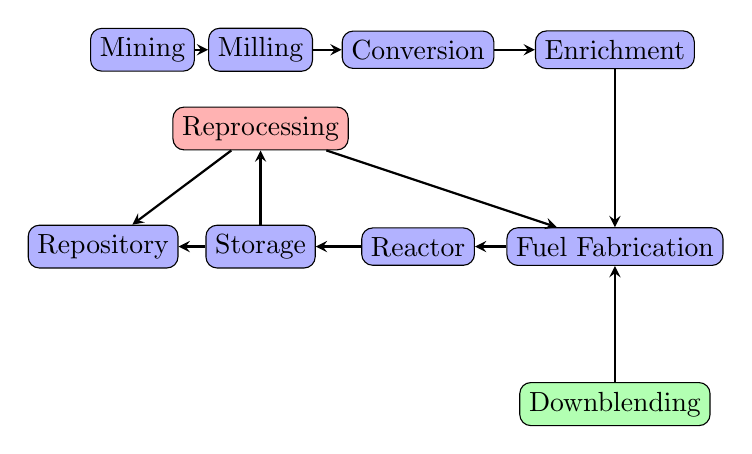
\begin{tikzpicture}[node distance=1cm]
        \node (mine) [agent] {Mining};
        \node (mill) [agent, right of=mine, xshift=0.5cm] {Milling};
        \node (conversion) [agent, right of=mill, xshift=1cm] {Conversion};
        \node (enrichment) [agent, right of=conversion, xshift=1.5cm]{Enrichment};
        \node (fabrication) [agent, below of=enrichment, yshift=-1.5cm]{Fuel Fabrication};
        \node (reactor) [agent, left of=fabrication, xshift=-1.5cm]{Reactor};
        \node (storage) [agent,  left of=reactor, xshift=-1cm]{Storage};
        \node (sinkhlw) [agent, left of=storage, xshift=-1cm]{Repository};


        \draw [arrow] (mine) --  (mill); 
        \draw [arrow] (mill) -- (conversion); 
        \draw [arrow] (conversion) -- (enrichment);
        \draw [arrow] (enrichment) -- (fabrication);
        \draw [arrow] (fabrication) -- (reactor);
        \draw [arrow] (reactor) -- (storage);
        \draw [arrow] (storage) -- (sinkhlw);
        \pause
        \node (reprocessing) [transition, above of=storage, yshift=0.5cm]{Reprocessing};
        
        \draw [arrow] (storage) -- (reprocessing);
        \draw [arrow] (reprocessing) -- (fabrication);
        \draw [arrow] (reprocessing) -- (sinkhlw);
        \pause
        \node (downblending) [region, below of=fabrication, yshift=-1cm]{Downblending};
        \draw [arrow] (downblending) -- (fabrication);

        \end{tikzpicture}
    \caption{Overview of the Nuclear Fuel Cycle.}
    \label{fig:fuel_cycle}
\end{figure}
\end{frame}

\begin{frame}
    \frametitle{Uranium enrichment}
    \begin{itemize}
        \item Process to increase the relative abundance of specific
              isotopes of an element
        \pause
        \item The throughput of a facility is based on the product 
              mass, product assay, and the \gls{SWU} capacity
    \end{itemize}
    \pause
    \vspace{-0.2cm}
    \begin{columns}
        \column{6.5cm}
            \begin{align*}
                    & F = P + T \\
                    & x_fF = x_pP + x_tT\\
                    & SWU = \left[P\times V(x_p) +T*V(x_t) - F*V(x_f)\right]*t\\
                    & \text{in which:}\\
                    & V(x_i) = (2x_i - 1)*\ln\left(\frac{x_i}{1-x_i}\right)
            \end{align*}
            \vspace{-0.5cm}
            \begin{figure}[t]
    \centering
    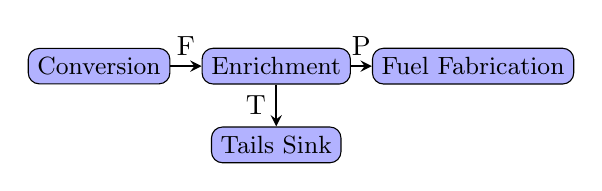
\begin{tikzpicture}[node distance=1cm]
        \node (conversion) [agent] {\small Conversion};
        \node (enrichment) [agent, right of=conversion, xshift=1.25cm]{\small Enrichment};
        \node (fabrication) [agent, right of=enrichment, xshift=1.5cm]{\small Fuel Fabrication};
        \node (sink) [agent, below of=enrichment]{\small Tails Sink};
        
        \draw [arrow] (conversion) -- node[anchor=south]{F} (enrichment);
        \draw [arrow] (enrichment) -- node[anchor=south]{P}(fabrication);
        \draw [arrow] (enrichment) -- node[anchor=east]{T}(sink);

        \end{tikzpicture}
\end{figure}
    \column{3.5cm}
    \begin{table}
        \centering
        \vspace{-0.3cm}
        \begin{tabular}{c m{2cm}}
            \hline
            Variable & Definition \\
            \hline
            F & feed mass \\
            P & product mass \\
            T & tails mass\\
            x$_i$ & assay of material stream \\
            SWU & Separative Work Units\\
            V(x$_i$) & separation potential function\\
            \hline
        \end{tabular}
    \end{table}

    \end{columns}
\end{frame}

\begin{frame}
    \frametitle{Efforts to estimate HALEU needs}
    Efforts are underway to estimate potential \gls{HALEU} needs:
    \begin{itemize}
        \item \gls{NEI} surveyed multiple reactor design companies
              to estimate \gls{HALEU} needs between now and 2035 
              \cite{korsnick_updated_2021,nuclear_energy_institute_establishing_2022}
        \item \gls{DOE} labs modeled the transition to some 
              \gls{HALEU}-fueled reactors to estimate \gls{HALEU} needs 
              to meet current net-zero carbon goals in 2050 \cite{dixon_estimated_2022}
    \end{itemize}
    This previous work is all based on announced advanced reactor projects.
\end{frame}

\subsection{Objectives}
\begin{frame}
    \frametitle{Technical gaps \& objectives}
    \begin{block}{Technical Gaps}
        \begin{itemize}
            \item Understand changes to the US nuclear fuel cycle to 
                  commercially supply \gls{HALEU}
            \item Understand limitations of using downblended \gls{HEU} 
                  in advanced reactors         
        \end{itemize}
    \end{block}
    \pause
    \begin{block}{Objectives}
        \begin{itemize}
        \item<2-> Explore how the deployment of \gls{HALEU}-fueled reactors 
        affects the US nuclear fuel cycle. 
        \item<2-> Quantify potential material requirements for the transition from 
              \glspl{LWR} to advanced reactors in a once-through and recycling 
              fuel cycle
        \item<2-> Understand the impacts of fuel cycle parameters on the 
              material requirements and design optimized transition scenarios
        \item<2-> Identify potential limitations in using downblended \gls{HEU} 
              in advanced reactors
        \end{itemize}
    \end{block}
\end{frame}
\section{Transition Analysis}
\input{transition_analysis}
\section{Results}
\input{results}
\subsection{Updated Methodology}
\begin{frame}
    \frametitle{Introduce and update capacity factors}
    The current methodology matches installed capacity to a demand 
    in the energy generated. Need to introduce capacity factors to 
    match energy generated to a demand in energy generated.
    \begin{itemize}
        \item Assume \glspl{LWR} operate at a 92.66\% 
              \gls{CF} \cite{us_eia_monthly_2022}
        \item Assume Xe-100 and VOYGR operate at 95\% \gls{CF}
              \cite{xenergy_reactor_nodate,nuscale_technology_nodate}
        \item Assume the \gls{MMR} operates at 100\% \gls{CF}
        \item Do not explicitly model outages for any reactor, extend 
              operating cycle by 1 month for \glspl{LWR} and VOYGRs
        \item This methodology changes the energy supplied by \glspl{LWR}, 
              slightly changes the number of reactors deployed,
              but does not affect the amount of fuel or when the reactors 
              receive fuel. 
    \end{itemize}
\end{frame}

\begin{frame}
    \frametitle{Effect of updated methodology}
    \begin{columns}
        \column[t]{5cm}
            \begin{itemize}
                \item The energy demand changes to 87.20 GWe-yr (previously 
                      89.46 GWe-yr) because 
                      of the updated LWR \gls{CF}
                \item All of the scenarios meet the minimum demand or 
                      provide an oversupply of power
                \item There is little variation in the energy supplied
                      in each scenario
            \end{itemize}
        \column[t]{5cm}
        \vspace{-0.8cm}
            \begin{figure}
                \centering
                \includegraphics[scale=0.4]{updated_energy_after_2025.pdf}
                \caption{Annual average energy produced (GWe-yr) in Scenarios 
                2-7 compared with energy demand}
                \label{fig:updated_energy}

        \end{figure}
    \end{columns}
\end{frame}

\subsection{Summary}
\begin{frame}
\frametitle{Summary}
Preliminary work investigates the material requirements 
of transitioning from \glspl{LWR} to different 
subsets of advanced reactors.
\begin{itemize}
        \item Primarily deploying VOYGRs increases the amount of 
              fuel required but decreases the mass of \gls{HALEU}
        \item Deploying primarily Xe-100s or VOYGRs results in 
              similar feed uranium and \gls{SWU} requirements
        \item Deploying \glspl{MMR} greatly increases the number of 
              reactors, feed uranium, and \gls{SWU} capacity required
        \item For a 1\% growth in energy demand, similar trends are 
              observed
\end{itemize}
However, the preliminary work has some limitations:
\begin{itemize}
        \item Only considers once-through fuel cycle
        \item Only considers changes in the energy demand and
              reactors deployed
        \item Only considers enriching natural uranium to produce 
              \gls{HALEU}
\end{itemize}
\end{frame}
\section{Proposed Work}
\begin{frame}
  \frametitle{Closed fuel cycle}
        \begin{columns}
        \column[t]{3.5cm}
        \begin{block}{Proposed Work}
                \begin{itemize}
                        \item Model the transition to advanced reactors using recycling
                        \begin{itemize}
                                \item Consider limited and continuous recycle
                                \item Quantify the same material requirements 
                        \end{itemize}
                \end{itemize}
        \end{block}
        \begin{block}{Technical Gap}
             \begin{itemize}
                \item Understand the effect of closing the nuclear fuel 
                      cycle on material requirements
             \end{itemize}                   
        \end{block}
        
        \column[t]{6.5cm}
        \input{recycle-flow}
        \end{columns}
\end{frame}

\begin{frame}
        \frametitle{Sensitivity analysis}
        \begin{block}{Proposed Work}
                \begin{itemize}
                        \item Perform sensitivity analysis on select once through 
                        and recycle transitions, changing three variables
                        \begin{itemize}
                                \item Transition start time
                                \item \gls{LWR} lifetimes
                                \item Build share of each advanced reactor
                        \end{itemize}
                        \item Optimize each the transitions investigated in the 
                                sensitivity analysis to minimize material requirements
                        \begin{itemize}
                                \item Two single-objective problems
                                \item One multi-objective problem
                        \end{itemize}
                \end{itemize}
        \end{block}
        \begin{block}{Technical Gap}
                \begin{itemize}
                        \item Understand how the transition start time, \gls{LWR} 
                                lifetime, and advanced reactor build share
                                affect the material requirements
                        \item Optimize transitions to minimize material requirements
                \end{itemize}
        \end{block}
\end{frame}

\begin{frame}
        \frametitle{Neutronics analysis}
        \begin{block}{Proposed Work}
                \begin{itemize}
                \item Perform depletion calculations of the Xe-100 and \gls{MMR} 
                        designs using different \gls{HALEU} compositions:
                        \begin{itemize}
                                \item Pure \gls{HALEU} (only $^{235}$U and $^{238}$U)
                                \item Downblended \gls{EBR} spent fuel
                                \item Downblended Y-12 stockpiles
                        \end{itemize}
                \item Investigate the reactor performance of each composition:
                        \begin{itemize}
                                \item Flux
                                \item Neutron multiplication ($k_{eff}$)
                                \item Delayed neutron fraction ($\beta_{eff}$)
                                \item Reactivity Coefficients
                        \end{itemize}
                \end{itemize}
        \end{block}
        \begin{block}{Technical Gap}
                \begin{itemize}
                        \item Understand the limitations 
                                of using \gls{HALEU} produced by downblending 
                                \gls{HEU} in the Xe-100 and MMR
                \end{itemize}
        \end{block}
\end{frame}

%\section{Conclusions}
%% General Summary


The goal of this work is to investigate the impacts of deploying reactors 
fueled 
by \gls{HALEU} in the United States, including the impacts that the reactors 
have on the \gls{NFC} and the impacts the \gls{NFC} has on the reactors. 
The results of this work are intended to
aid and guide policy makers and key stake holders on how to best establish a 
fuel cycle to support the deployment of \gls{HALEU}-fueled reactors. 
Within this primary goal, there are three specific objectives:
\vspace{0.2cm} 
\noindent
\begin{enumerate}
\item Quantify potential material requirements for the transition 
from \glspl{LWR} to advanced reactors in open and closed 
fuel cycles.

\item Understand the impacts of fuel cycle parameters on the material 
requirements and design optimized transition scenarios.

\item Identify potential limitations in using downblended \gls{HEU} 
on reactor performance.

\end{enumerate}

These goals were met by designing and modeling various transitions 
to advanced reactors, considering a once-through and a closed 
fuel cycle. The once through fuel cycles were then investigated 
further by performing sensitivity analysis and optimization. Finally, 
models of two different \gls{HALEU}-fueled advanced reactors were 
created to investigate the impact of different uranium isotopic 
compositions of the \gls{HALEU} fuel on reactor performance. 

% Once-through analysis

% Closed fuel cycle analysis

% Sensitivity analysis
Chapter 6 examined the effects of different input parameters for 
their effects on different output metrics for the fuel cycle transition from 
\glspl{LWR} to different advanced reactors. The \gls{OAT} analysis identified the 
trends from varying each input parameter independently, and how the deployment 
scheme for this work impacts each of the results. The analysis also 
identified tradeoffs between different reactor designs, such as how the Xe-100 
needs more \gls{HALEU} than the VOYGR, but a smaller fuel mass. The synergistic 
analysis identified how some of the input parameters interact to affect the output 
metrics. While some of the combinations of input parameters (e.g., varying 
the \gls{LWR} lifetime and the VOYGR build share) had consistent trends 
across the input parameter space, some combinations (e.g., varying the Xe-100 
burnup and the \gls{MMR} share) varied in their effect across the input parameter 
space. Finally, the global sensitivity analysis quantified the effect of different 
input parameters on the output metrics. We build surrogate models to fully capture 
the input parameter space. The models were consistent with the Sobol' indices, 
such that the Xe-100 burnup is the most impactful parameter when varying any 
of the three advanced reactor build shares. 

% Optimization
Chapter 7 demonstrated a methodology to optimize the once-through 
transitions and identified transitions that minimize different 
fuel cycle metrics. Results from this chapter show that minimizing the 
\gls{SWU} capacity to produce \gls{HALEU} requires maximizing the number of 
VOYGRs built, minimizing the mass of \gls{SNF} requires maximizing the number 
of Xe-100s built, and minimizing both of these fuel cycle metrics is a 
balance between deploying Xe-100s and VOYGRs. The results from the optimization 
work was consistent with the results of the sensitivity analysis, but 
they did not fully meet expectations. The input parameters identified that 
were not subject to a linear constraint (i.e., not the advanced reactor 
build shares) matched expectations based on the trends of the sensitivity 
analysis and intuition. However, The methodology employed for this 
analysis did not adhere well to the linear constraint of the advanced reactor 
build shares in all three of the problems. Therefore, the 
results from the optimization work can not be taken at face value 
and are better used to identifying a relationship between the advanced 
reactor build shares than a specific set of parameters. 


% Neutronics
 
\section{Future Work}
The work performed here provides a foundation for continued analysis and 
exploration of the fuel cycle impacts of deploying \gls{HALEU}-fueled reactors. 
Potential areas of future work include modeling non-fuel materials needed 
to support these transitions, such as the amount of reactor-grade graphite 
to be the moderators in the Xe-100 and \gls{MMR}. This analysis would 
provide insight into other supply chain requirements that equally 
impactful on establishing these fuel cycles. Additionally, the 
results of this work can be used to determine facility sizes, throughputs, 
and numbers. This information aids in developing the supply chains 
to support these transitions, but also in designing and evaluating 
safeguards for these transitions. Potential safeguards measures may 
limit the facility sizes and the amount of material that can move from 
one facility to another, which affects how the transition can be 
implemented. By 
incorporating facility information into the fuel cycle model, the 
sensitivity analysis and optimization methodologies can be used 
to identify ways to adjust the transition to better account for 
the facility limitations and safeguards needs. 

The analysis of the downblended \gls{HEU} on the reactor performance
can also be expanded. For example, consider other \gls{HALEU}-fueled 
reactors, such as the Oklo Aurora, that have announced an intent to 
use \gls{HALEU} created from these stockpiles. Additionally, expand 
the analysis to other metrics, such as power peaking factors and 
power distributions in the core, or 
increase the fidelity of the models. Ways to increase the model 
fidelities include incorporating burnable poisons, control rods, 
and couple with heat transfer calculations to create a multi-physics model. 
These incorporations into the models will provide greater 
accuracy to the results. 
\begin{frame}
    \frametitle{Acknowledgements}
    This material is based upon work supported under a University 
    Nuclear Leadership Program Graduate Fellowship. Any opinions, findings, conclusions, or 
recommendations expressed in this publication are those of the author(s) 
and do not necessarily reflect the views of the Department of Energy Office 
of Nuclear Energy.

\end{frame}


\begin{frame}[allowframebreaks]
    \frametitle{References}
    \bibliographystyle{plain}
    {\footnotesize \bibliography{../bibliography} }
  
  \end{frame}
\begin{frame}
    \frametitle{Summary}
    \begin{columns}
      \column[t]{5cm}
      \begin{itemize}
        \item Investigating the transition to \gls{HALEU}-fueled reactors
        \item Results show primarily deploying VOYGRs increases the mass 
              of enriched uranium required
        \item Feed uranium required is similar order of magnitude to \gls{LWR}
              requirements unless transitioning to only \gls{MMR}
        \item Expand work to include closed fuel cycles, sensitivity 
              analysis, and neutronics effects of downblened \gls{HEU}
      \end{itemize}

      \column[t]{5cm}
        \begin{figure}[t]
          \includegraphics[scale=0.35]{nogrowth_AR_uranium.pdf}
        \end{figure}
        
    \end{columns}
    
\end{frame}


\begin{frame}
    \frametitle{Once-through feed uranium}
    \begin{figure}
        \centering 
        \includegraphics[scale=0.5]{nogrowth_feed.pdf}
    \end{figure}
\end{frame}

\begin{frame}
    \frametitle{Recycle HLW}
    \begin{figure}
        \centering
        \includegraphics[scale=0.5]{nogrowth_recycle_hlw.pdf}
    \end{figure}
\end{frame}

\begin{frame}
    \frametitle{Recycle SNF}
    \begin{figure}
        \centering
        \includegraphics[scale=0.3]{nogrowth_recycle_snf.pdf}
    \end{figure}
\end{frame}

\begin{frame}
    \frametitle{Recycle SWU}
    \begin{figure}
        \centering
        \includegraphics[scale=0.3]{nogrowth_recycle_swu.pdf}
    \end{figure}
\end{frame}

\begin{frame}
    \frametitle{Effects of varying VOYGR build share}
    \begin{figure}
        \centering
        \includegraphics[scale=0.5]{voygr.pdf}
    \end{figure}
\end{frame}

\begin{frame}
    \frametitle{Effects of varying MMR build share}
    \begin{figure}
        \centering
        \includegraphics[scale=0.3]{mmr.pdf}
    \end{figure}
\end{frame}

\begin{frame}
    \frametitle{Axial flux through Xe-100}
    \begin{figure}
        \centering 
        \begin{subfigure}{0.49\textwidth}
            \includegraphics[scale=0.35, trim=20 10 10 20,clip]{xe100_thermal_axial.pdf}
        \end{subfigure}
        \begin{subfigure}{0.49\textwidth}
            \includegraphics[scale=0.35, trim=10 10 10 20,clip]{xe100_fast_axial.pdf}
        \end{subfigure}
        \caption{Axial fluxes through Xe-100.}
        \label{fig:xe100-axial-flux}
    \end{figure}
\end{frame}

\begin{frame}
    \frametitle{Reactivity feedback coefficients for Xe-100}
    \begin{table}[ht]
        \centering
        \caption{Reactivity temperature feedback coefficients for 
        each material type in the Xe-100-like model for each fuel 
        type.}
        \label{tab:coeff_xe100}
        \begin{tabular}{c c c c c}
            \hline 
            & \multicolumn{4}{c}{Material feedback coefficient (pcm/K)} \\
            Fuel Type & Fuel & Coolant & Moderator & Total \\
            \hline
            Pure & -3.875 $\pm$ 0.094 & -0.044 $\pm$ 0.112 & -0.071 $\pm$ 0.459 & -4.216 $\pm$ 0.502\\
            \gls{EBR} & -3.759 $\pm$ 0.138 & -0.433 $\pm$ 0.048 & -0.708 $\pm$ 0.404 & -4.817 $\pm$ 0.438\\
            Y-12 & -3.797 $\pm$ 0.157 & -0.351 $\pm$ 0.092 & -0.728 $\pm$ 0.469 & -4.700 $\pm$ 0.349\\
            \hline

        \end{tabular}
\end{table}
\end{frame}

\end{document}
